\section{Columnar Data Storing}

The final stage of any data analysis is representing the data in a columnar format and fetching some subset of the data with constraints 
on other columns. At this stage, users operate on a large data set with many columns and rows, and access to all of the 
columns in the file is not required. The Apache Parquet~\cite{PARKQUET:2020jk} format is widely used in data science for storing columnar data, due to its tools
with Python data frames. It is highly tuned to store large data sets and provide fast access to required columns. The Parqute is gaining
some popularity in High Energy and Nuclear Physics with the growing popularity of Python as a physics analysis environment. In the
past two decades, the ROOT was the primary tool for physics analysis which also provides data structures for storing columnar data 
and accessing the columns selectively. It is worth mentioning that ROOT also has Python bindings. To extend the usage of HiPO files beyond
the data processing int physics analysis, and experimental implementation of columnar data storage were implemented and tested against the more established data formats.

\subsection{Design}

The flexibility of the HiPO data format allows storing data in columnar format, similar to Parquete and ROOT. 
The feature of assigning tags to records allows for writing the data in a columnar manner, where each column is assigned a tag and written separately into its own record.
This process is synchronized so that at every predetermined number of rows, every column data is serialized and outputted as a record. The schematic view of arranging 
the data in the file is shown in Figure~\ref{fig:tuple_schema}.

\begin{figure}[h!]
  \begin{center}
    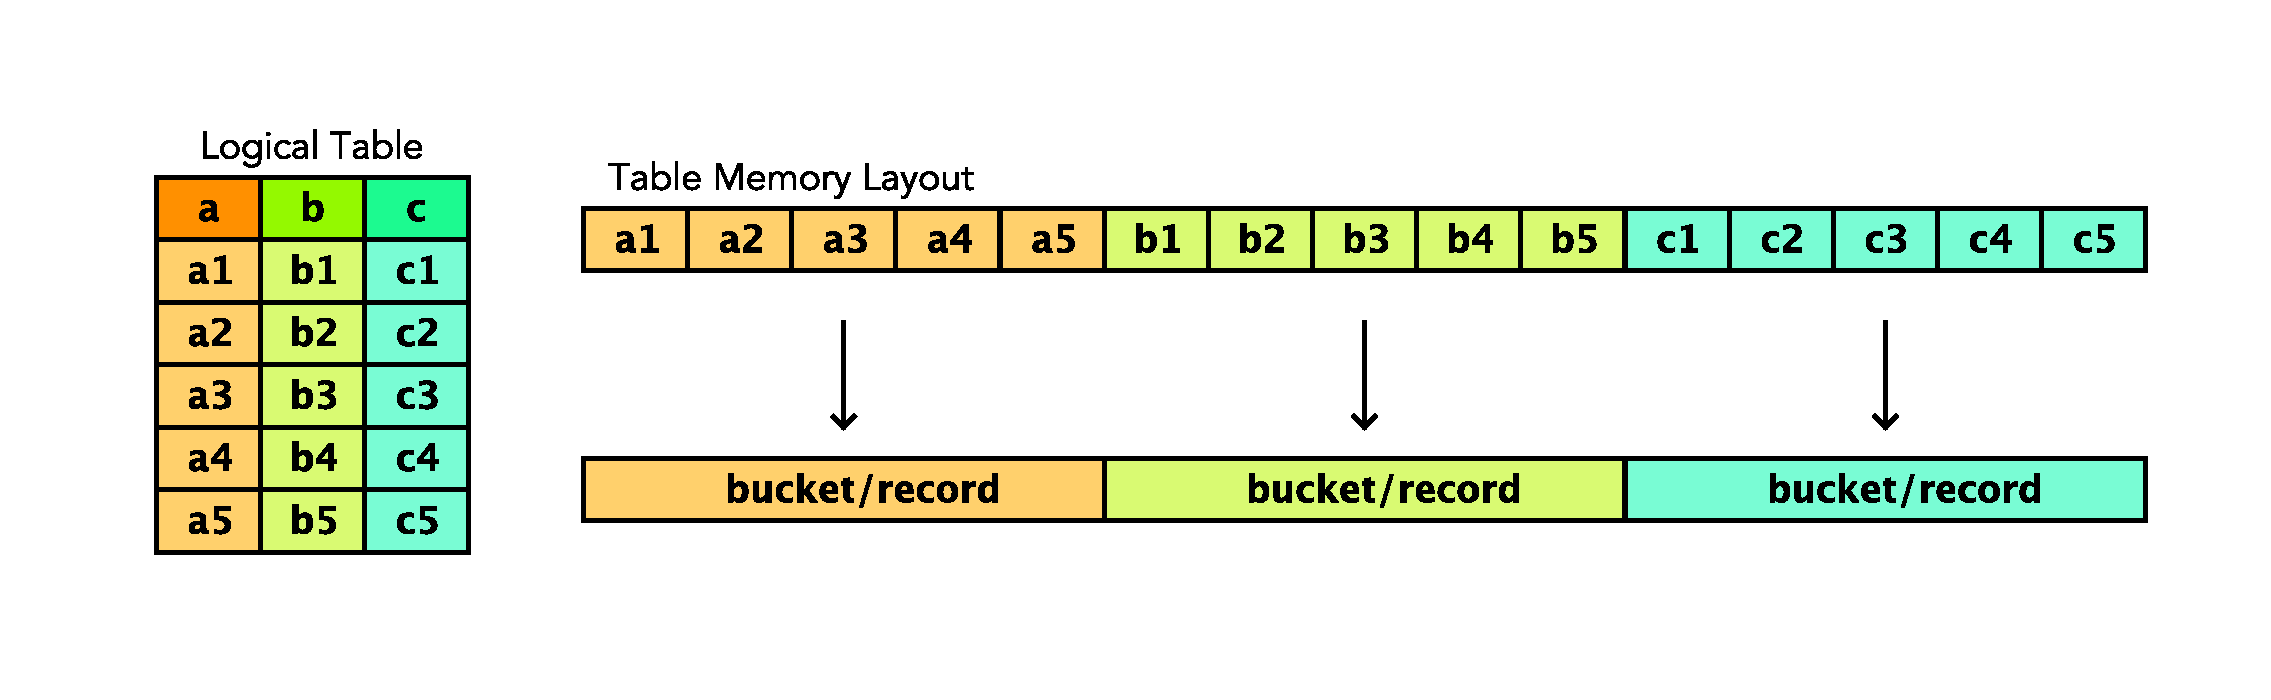
\includegraphics[width=0.85\textwidth]{images/tuple_schema.pdf}
 \end{center}
  \caption{Schematic view of arranging each event in the file from columnar table.}
 \label{fig:tuple_schema}
\end{figure}

When reading the file, the desired columns (called branches) are declared, and only records (buckets) with corresponding tag numbers are read and deserialized.
The user program has access only to the declared branches. The files written as columnar data have to be read with the corresponding API to make sure that the columns 
are properly synchronized at the read time. Here is an example code to read a few columns from a file and fill in a histogram. 
%\begin{verbatim}
%\rule{16.5cm}{0.4pt}
\begin{lstlisting}[language=c++, caption=c++ example to read HiPO tuple file and fill a histogram., label=lst:read_tuple]
// open file and read-only specified branches
hipo::tuple tuple("tuple.h5", "c1:c2:c3:c4"); 
float data[4]; // declare a holder for the data to be read
twig::h1d h(120,-1.0,1.0); // declare a histogram
while(tuple.next(data)==true){
    h.fill(data[0]);
}
\end{lstlisting}
%\end{verbatim}

The example code shown on Listing~\ref{lst:read_tuple} opens a file to read branches names "c1"-"c4" from the file, reads all rows until reaching the end of the file passing them to the user code through a declared array. The values from the first branch ("c1") will be filled into a histogram.

\subsection{Benchmarking}

For reading tests, we produced a synthetic data set consisting of 24 columns and 50 M rows and created HiPO (4.8 GB), ROOT (4.4 GB), and Parquete (5.1 GB) files, all three with LZ4 compression. The columns were filled with randomly generated numbers in the range $0..1$. 

\begin{figure}[h!]
  \begin{center}
    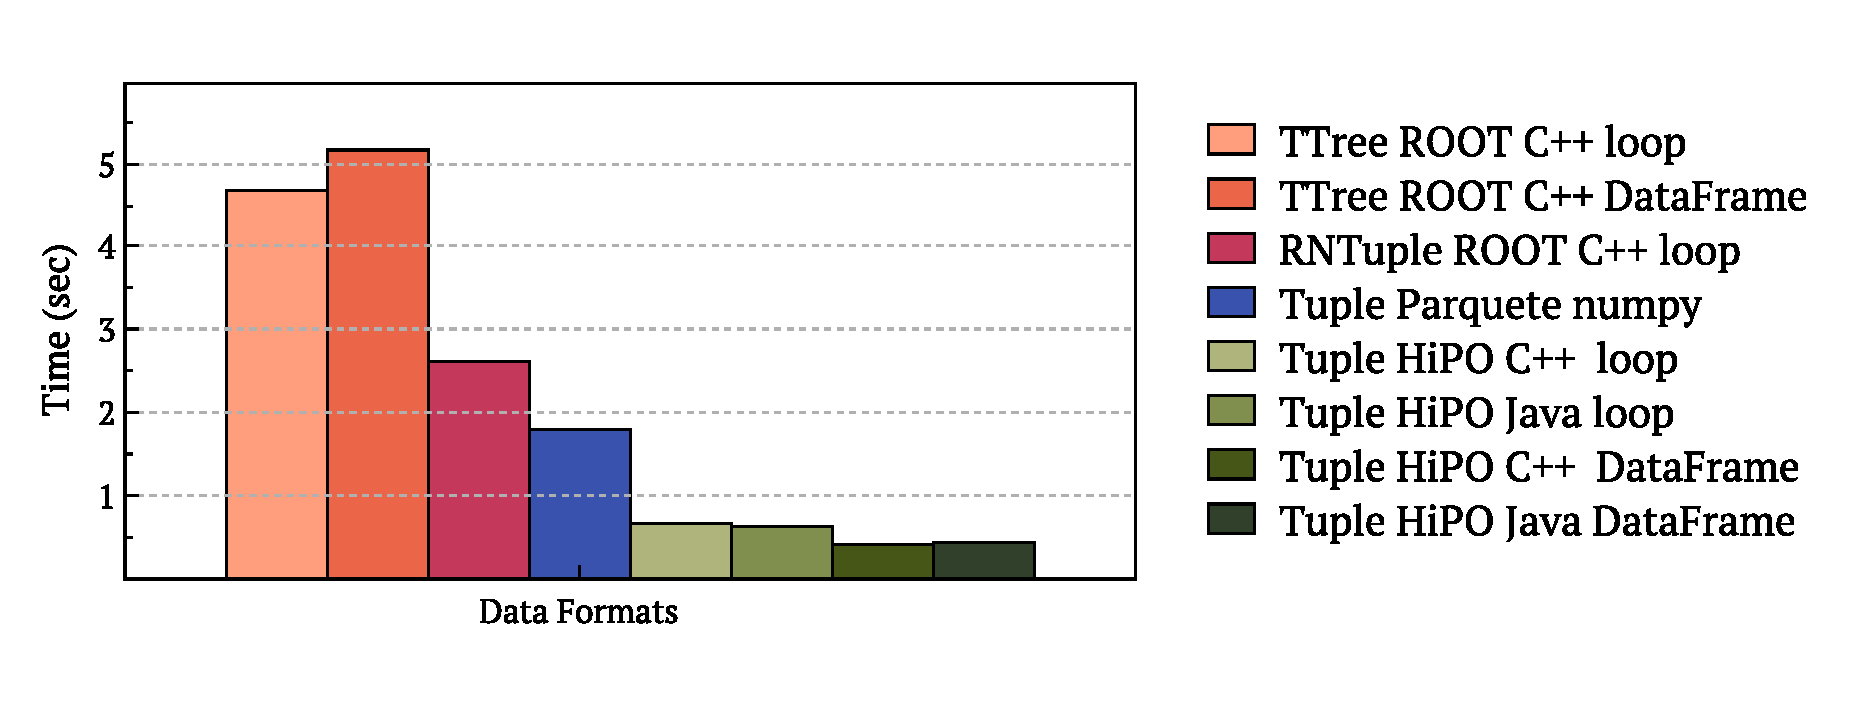
\includegraphics[width=0.85\textwidth]{images/benchmark_final.pdf}
%     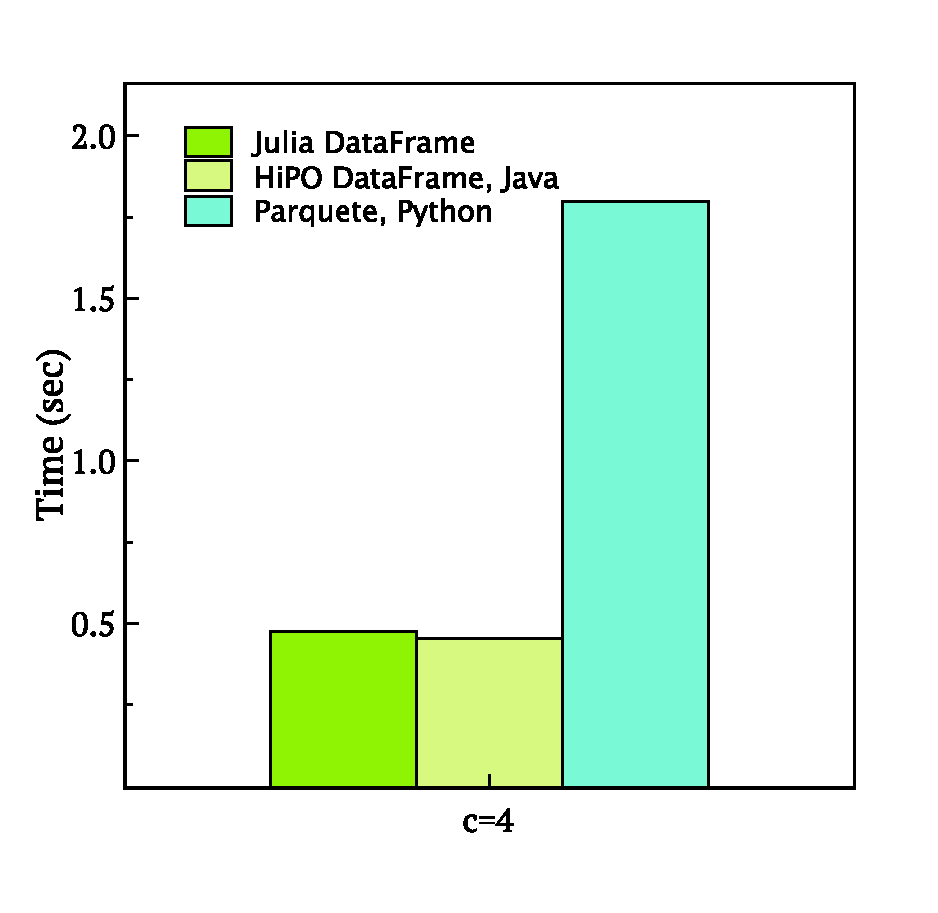
\includegraphics[width=0.45\textwidth]{images/data_frame_benchmark.pdf}
 \end{center}
  \caption{Reading benchmark for different file formats reading the columnar data with 24 columns and 50 M rows (file size $\approx 4.5 GB$). Only four columns are read, and histograms are filled for the respective columns. }
 \label{read_benchmark}
\end{figure}

Then, reading tests were performed by reading four branches (out of 24) from the data file and filling a histogram for each branch, representing a typical workflow for data exploration. The times were measured for ten consecutive reads, and the average time of the last four reads was used as the final result. The results are shown in Figure~\ref{read_benchmark}. As can be seen from the figure, the ROOT TTree has the worst performance however, the RNTuple, which is the new data format standard in the upcoming ROOT 7 release, provides significant improvements in data reading speeds, and its performance is similar to that of Paruet. 


\begin{table}[h!]
\centering
%\begin{tabular}{|l|c|c|c|c|} % '|' for borders, 'c' for center alignment
\begin{tabular}{|p{7cm}|p{3.0cm}|p{4.0cm}|}
\hline
\textbf{Format (Library)} & File Size (GB)  &  Execution time (sec)  \\ \hline \hline
Tuple HiPO Java loop      & 4.8&0.637 \\ \hline
Tuple HiPO Java DataFrame &4.8& 0.452 \\ \hline
Tuple HiPO C++  loop      &4.8& 0.675 \\ \hline
Tuple HiPO C++  DataFrame &4.8& 0.424 \\ \hline
Tuple HiPO Julia  DataFrame &4.8& 0.487 \\ \hline
Tuple Parquete DataFrame  &5.1& 1.812 \\ \hline
TTree ROOT C++ loop       &4.4 & 4.692 \\ \hline
TTree ROOT C++ DataFrame  &4.4 & 5.175 \\ \hline
RNTuple ROOT C++ loop     &3.8& 2.624 \\ \hline
RNTuple ROOT C++ loop (CINT)    &3.8&  5.283 \\ \hline
%--- 6.32 RNTuple ROOT C++ loop     &3.8& 1.843 \\ \hline
%--- 6.32 RNTuple ROOT C++ loop (CINT)    &3.8&  3.861 \\ \hline
Tuple HiPO Java loop (JShell)  &4.8&  0.672 \\ \hline
%ROOT TTree (C++)  &  4.4 GB & 106.40 & 5.37 sec&10.10 sec& 14.35 sec       \\ \hline
%HiPO Tuple   (C++)   & 4.8 GB & -  & 1.35 sec & 2.61 sec & 4.22 sec       \\ \hline
%HiPO Tuple  (Java)   & 4.8  GB & 5.82 & 2.16 sec & 3.78 sec & 5.84 sec     \\ \hline
%Parquete (Python)     &  5.1 GB & 15.97 & 1.80 sec & 3.56 sec & 5.44 sec        \\ \hline
%DataFrames (Julia)   &  4.8 GB & - & 0.48 sec & 0.70 sec & 0.96 sec      \\ \hline
%DataFrames  (Java)   & 4.8  GB & 5.82 & 0.35 sec & 0.53 sec& 0.57 sec   \\ \hline
%DataFrames  (C++)   & 4.8  GB & 5.82 & 0.55 sec & 0.73 sec& 0.94 sec   \\ \hline
\end{tabular}
\caption{Reading benchmark for different file formats reading four columns from a file and filling respective histograms for each column. The file is generated with 24 columns and 50M rows filled with random numbers [0..1]. }
\label{tab:read_benchmark}
\end{table}

The numerical values for these tests are summarized in Table~\ref{tab:read_benchmark}. 
The HiPO data format provides much faster reading speeds compared to Parquet and ROOT (RNtuple) in simple reading the data in the loop (as shown in Listing~\ref{lst:read_tuple}), both in C++ and Java implementations. The "DataFrame" in the tests indicates the experimental feature of HiPO where the histogram is passed to the tuple reader, and it uses bulk histogram fill from the data buckets, it provides $50\%$ improvement in filling the histograms.
The table also contains the preliminary benchmark in the Julia port of the HiPO library (not included in the graph), showing performance similar to compiled C++ code.

One thing to mention is that most of the exploratory data analysis is done in interactive shells using ROOT files where various combinations of selections can be used to plot selected variables. Our tests showed that the RNTuple performance drops significantly when using it in interactive mode (by a factor of 2), while using the HiPO Java library in interactive JShell does not affect the performance (seen in Table~\ref{tab:read_benchmark}). 
The columnar storage in HiPO is experimental, and the C++ source will be made public after intensive debugging. The Java code is available in the repository to run preliminary benchmarks.
%The numerical values for these tests are summarized in Table~\ref{tab:read_benchmark}. It is important to note that the writing performance of the data format is very important if it will be used in online for storing the experimental data. The faster serialization is preferable for the choice of data format. The writing times for the different formats are also summarized in Table~\ref{tab:read_benchmark}, and as it can be seen the writing times for HiPO are significantly shorter compared to both ROOT and Parquete.

%The benchmarks shown in Figure~\ref{read_benchmark} are performed using a loop over all elements in the tuple, where after each loading of the data, the control is returned to the user code where the histogram is filled (for ROOT and HiPO tuples). However, the Parquete (Python) code uses bulk fill when the histogram is filled from the data frame. This considerably speeds up the execution time due to reduced function calls. To have a fair comparison with the Parquet format in the HiPO library, bulk fill of histograms was implemented (both in Java, C++, and Julia), and the same tests were performed using bulk fill. The results of reading four columns and bulk-filling the values into histograms are shown in Figure~\ref{read_benchmark} (b). The comparison shows that HiPO is $4-5$ times faster than Parquet and about 10-15 times faster than reading four columns in ROOT.

The benchmarks are performed on an M1 Macbook Laptop with a 1 TB SSD drive, using JDK 21 for Java library and ROOT 6.34.08.
